% Forward and reverse mode on the same computational graph. Left: every node
% carries its primal and its tangent, and both move forward together, in one
% pass. Right: a forward pass computes the primals and keeps them, then a
% backward pass takes the cotangents from the result back to the arguments;
% x_1, used by two steps, sums what both pass it.
% Build: see figures/README.md
\documentclass[tikz, border = 6pt]{standalone}
\usepackage[T1]{fontenc}
\usepackage{lmodern}
\usepackage{amsmath}
\usetikzlibrary{calc, arrows.meta, shapes.multipart, decorations.pathreplacing}

\definecolor{primal}{HTML}{8A8A8A}
\definecolor{tang}{HTML}{2A7AB0}
\definecolor{cotang}{HTML}{C0622B}

\newcommand{\pr}[1]{\textcolor{primal}{#1}}
\newcommand{\tg}[1]{\textcolor{tang}{#1}}
\newcommand{\ct}[1]{\textcolor{cotang}{#1}}

\tikzset{
  >={Stealth[length = 2mm]},
  val/.style = {circle split, draw = black!55, minimum size = 12mm, inner sep = 1.5pt,
    font = \small, path picture = {\fill[#1!10] (path picture bounding box.west)
      rectangle (path picture bounding box.south east);}},
  flow/.style = {->, thick, shorten <= 6.4mm, shorten >= 6.4mm},
  pass/.style = {-{Stealth[length = 3mm, width = 3mm]}, line width = 2.5pt},
  passlabel/.style = {font = \footnotesize, anchor = north west, inner sep = 0pt, align = left},
  brace/.style = {decorate, decoration = {brace, amplitude = 5pt}, black!55, thick},
  side/.style = {font = \small, align = left, inner sep = 0pt},
  title/.style = {font = \bfseries, anchor = south west, inner sep = 0pt}
}

% An edge from #1 to #2: the primal forward and, beside it, the tangent forward.
\newcommand{\edgefwd}[2]{
  \draw[flow, primal] ($(#1)!3pt!90:(#2)$) -- ($(#2)!3pt!-90:(#1)$);
  \draw[flow, tang] ($(#1)!3pt!-90:(#2)$) -- ($(#2)!3pt!90:(#1)$);
}
% An edge from #1 to #2: the primal forward and, beside it, the cotangent backward.
\newcommand{\edgerev}[2]{
  \draw[flow, primal] ($(#1)!3pt!90:(#2)$) -- ($(#2)!3pt!-90:(#1)$);
  \draw[flow, cotang] ($(#2)!3pt!90:(#1)$) -- ($(#1)!3pt!-90:(#2)$);
}

\begin{document}
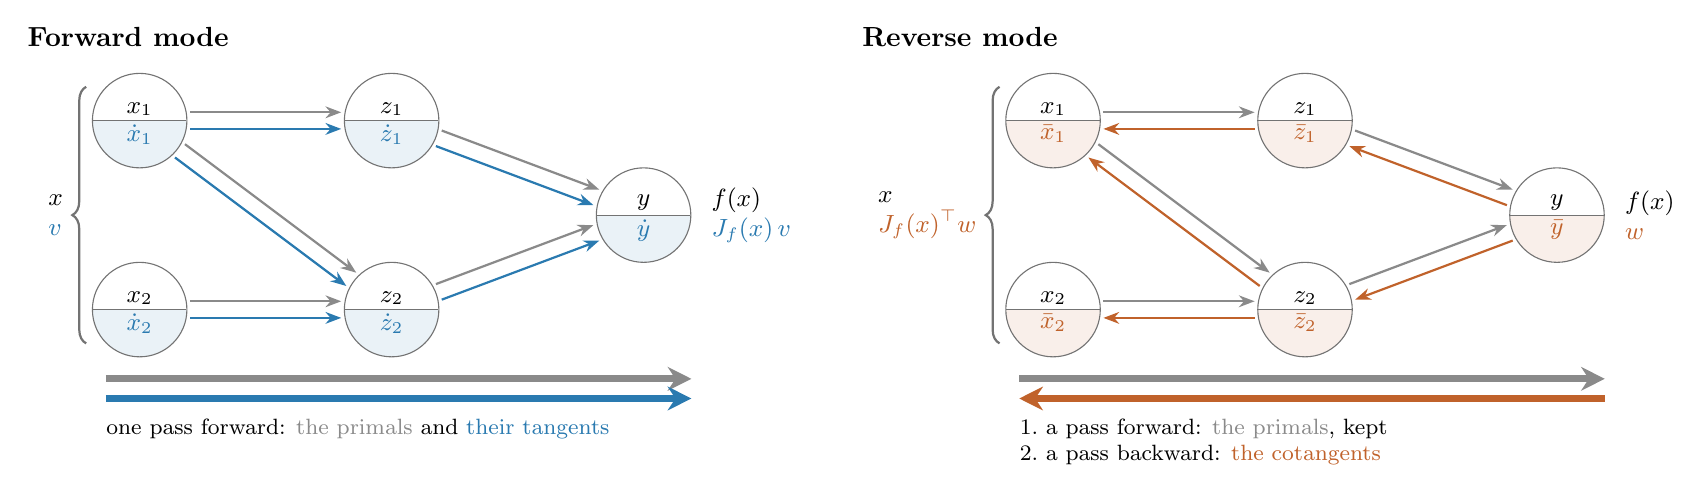
\begin{tikzpicture}

  % ---- forward mode -------------------------------------------------------
  \node[val = tang] (fx1) at (0, 1.2) {$x_1$\nodepart{lower}\tg{$\dot x_1$}};
  \node[val = tang] (fx2) at (0, -1.2) {$x_2$\nodepart{lower}\tg{$\dot x_2$}};
  \node[val = tang] (fz1) at (3.2, 1.2) {$z_1$\nodepart{lower}\tg{$\dot z_1$}};
  \node[val = tang] (fz2) at (3.2, -1.2) {$z_2$\nodepart{lower}\tg{$\dot z_2$}};
  \node[val = tang] (fy) at (6.4, 0) {$y$\nodepart{lower}\tg{$\dot y$}};

  \edgefwd{fx1}{fz1}
  \edgefwd{fx1}{fz2}
  \edgefwd{fx2}{fz2}
  \edgefwd{fz1}{fy}
  \edgefwd{fz2}{fy}

  \draw[brace] ($(fx2.south west) + (-0.25, 0)$) -- ($(fx1.north west) + (-0.25, 0)$)
    node[side, text = black, midway, anchor = east, xshift = -8pt] {$x$\\\tg{$v$}};
  \node[side, anchor = west] at ($(fy.east) + (0.25, 0)$) {$f(x)$\\\tg{$J_f(x)\,v$}};

  \node[title] at ($(fx1.north west) + (-1.0, 0.5)$) {Forward mode};

  \draw[pass, primal] ($(fx2.south west) + (0, -0.45)$) -- ($(fx2.south west -| fy.east) + (0, -0.45)$);
  \draw[pass, tang] ($(fx2.south west) + (0, -0.7)$) -- ($(fx2.south west -| fy.east) + (0, -0.7)$);
  \node[passlabel] at ($(fx2.south west) + (0, -0.95)$)
    {one pass forward: \pr{the primals} and \tg{their tangents}};

  % ---- reverse mode -------------------------------------------------------
  \begin{scope}[xshift = 11.6cm]
    \node[val = cotang] (rx1) at (0, 1.2) {$x_1$\nodepart{lower}\ct{$\bar x_1$}};
    \node[val = cotang] (rx2) at (0, -1.2) {$x_2$\nodepart{lower}\ct{$\bar x_2$}};
    \node[val = cotang] (rz1) at (3.2, 1.2) {$z_1$\nodepart{lower}\ct{$\bar z_1$}};
    \node[val = cotang] (rz2) at (3.2, -1.2) {$z_2$\nodepart{lower}\ct{$\bar z_2$}};
    \node[val = cotang] (ry) at (6.4, 0) {$y$\nodepart{lower}\ct{$\bar y$}};

    \edgerev{rx1}{rz1}
    \edgerev{rx1}{rz2}
    \edgerev{rx2}{rz2}
    \edgerev{rz1}{ry}
    \edgerev{rz2}{ry}

    \draw[brace] ($(rx2.south west) + (-0.25, 0)$) -- ($(rx1.north west) + (-0.25, 0)$)
      node[side, text = black, midway, anchor = east, xshift = -8pt] {$x$\\\ct{$J_f(x)^\top w$}};
    \node[side, anchor = west] at ($(ry.east) + (0.25, 0)$) {$f(x)$\\\ct{$w$}};

    \node[title] at ($(rx1.north west) + (-2.0, 0.5)$) {Reverse mode};

    \draw[pass, primal] ($(rx2.south west) + (0, -0.45)$) -- ($(rx2.south west -| ry.east) + (0, -0.45)$);
    \draw[pass, cotang] ($(rx2.south west -| ry.east) + (0, -0.7)$) -- ($(rx2.south west) + (0, -0.7)$);
    \node[passlabel] at ($(rx2.south west) + (0, -0.95)$)
      {1.\ a pass forward: \pr{the primals}, kept\\
       2.\ a pass backward: \ct{the cotangents}};
  \end{scope}

\end{tikzpicture}
\end{document}
